% !Mode:: "TeX:UTF-8"

%%%中文版式与英文版式通过参数设置
\documentclass{ctacn}%英文版式

%可以选择使用times字体
\usepackage{newtxtext}
\usepackage{hhline}
\usepackage{ctex}

\begin{document}


%%%%%%%输入年、月、卷、期
\Volume{xxxx}{x}{xxx}{xx}{x}
\cndoi{1001-0920(0000)00-0000-00}
\doi{10.13195/j.kzyjc.0000.0000}
\paperdate{xxxx-xx-xx}{xxxx-xx-xx}%接收日期,修回日期
%%%%%%%设置开始页
\setcounter{page}{1}

%%%%%%%输入页眉显示的题目

%%%%%%%%%%
%%%                  本刊为匿名审稿,新投稿时不要填写任何作者信息,包括所有位置的姓名、单位以及邮箱
%%%%%%%%%%%%
\runheading{基于加入DropOut的降噪自编码的磨矿系统故障诊断}%页眉设置,填写第一作者及论文题目
\xiangmujijin{国家自然基金项目(00000000)}%项目基金  为空会自动取消显示
\authorintro{作者一\,(1974$-$), 男, 教授, 博士, 从事XXX及其应用等研究;作者(1990$-$), 男, 硕士生, 从事XXX的研究.}%作者简介,填写第一作者和导师的简介         %新投稿不修改
\authorcor{E-mail: zuozheyi@163.com}%通讯作者邮箱,新投稿不修改

%%%-------------中文信息---------------
\cntitle{基于加入DropOut的降噪自编码的磨矿系统故障诊断} %输入中文标题


%                  新投稿不要修改下面的姓名及单位
%%%中文作者和单位,\dag代表通信作者,“作者一”代表3个字的名,“作者”代表2个字的名
\cnauthor{作者一\makebox{$^{1,2\dag}$},~~作~~~~者\makebox{$^{1}$}}%新投稿不修改
{(1. 东北大学~信息科学与工程学院,沈阳~110004;2. 曲阜师范大学~工学院, 山东~日照~276826)}%%省会城市无需加省%%新投稿不要修改

%%%中文摘要
\cnabstract{目前磨矿系统故障诊断多为人为判断,然而磨矿系统的数据较复杂,与故障发生并没有十分具体的联系,人为判断困难重重。而磨矿系统的数据对于常规机器学习算法来说大多面临着线性不可分的困难。为了解决线性不可分问题,我们使用人工神经网络进行故障分类,但面对复杂的故障数据,神经网络表达能力有限,为了增强表达能力,使用自动编码器增加网络深度,并使神经网络可以快速收敛。然而,自动编码器遇到了严重的过拟合现象,因此使用加入DropOut的降噪自编码,最终加入DropOut的降噪自编码网络对于故障的分类准确率达到93.7\%。}

%%%中文关键词
\cnkeyword{故障诊断;自动编码器;DropOut;降噪自编码;Softmax分类器;深度学习}

%%%分类号、标识码
\clc{TP273}%中文分类号
\wenxianbiaoshi{A}%文献标志码

%%%%%%%----------------英文信息------------
\entitle{The Guide of the \LaTeX{} Template for preparing the manuscript of Control and Decision}


%%%%%%%              新投稿不要修改下面的英文名及单位
\enauthor{ZUO Zhe-yi\makebox{$^{1,2\dag}$},~~ZUO Zhe\makebox{$^{1}$}}{
(1. College of Information Science and Engineering,Northeastern University,Shenyang~110004,China;2. College of Engineering, Qufu Normal University,Rizhao~276826,China)}


\enabstract{ This article is designed to help in the contribution for Control and Decision. It is divided into several sections. It
consists of the styles and notes for the main text, the mathematical writing style and the topic of drawing tables and inserting
figures respectively. The residuals deal with references, acknowledges, etc.}

\enkeyword{Key word1;Key word2;Key word3;Key word4}

\maketitle




\begin{multicols}{2}
\section{引\quad 言}
磨矿过程是选矿厂生产过程的最重要环节之一,其主要任务是将矿石经过物理的研磨和分级,使有用矿物与脉石单体解离,为后续的选别作业创造条件。

磨矿过程是典型的流程工业过程,生产过程缓慢,滞后时间长,其机理复杂、影响因素多,如给矿量、给水量、原矿性质及装球量等随机变化及各种外界干扰因素,往往造成磨矿过程工作不稳定。现有磨矿分级过程核心设备球磨机的运行监控还仅仅停留在对数据的显示和存储上,没有完整的故障诊断系统为设备的稳定运行保驾护航,根本原因也在于人员因素和技术因素,矿山环境大多恶劣偏僻,难以吸引专业技术人员,而故障诊断的基础是通过操作人员的经验积累人工判断来实现的,而人为控制的过程由于受到种种外界条件的干扰,会对控制结果产生直接或间接的影响。

近年来,网络及数据分析诊断理论的应用越来越发达,通过物联网对现场数据进行传送至生产制造企业,如何通过采集到的现场数据进行挖掘分析,实现高效的故障诊断系统越来越得到矿山生产单位的关注与期待。

本文基于以上问题,使用加入DropOut的降噪自编码算法,实现对V型磨矿系统工作过程中故障智能诊断。

本文首先对采集点长期以来采集到的数据集,对其进行数据预处理:确定输入向量维度、补全缺失数据、清洗噪声数据、定义故障表征方法,并进行数据关联分析建立起样本数据中特征向量与标签数据之间的映射关系。

接下来,搭建传统BP神经网络设置网络参数,输入为没有进行任何特征变换的特征向量,训练网络最终输出的结果效果并不好,可以发现对于高维输入特征向量传统BP神经网络收敛速度慢且辨识效果差。

为了解决传统BP神经网络对高维输入特征向量辨识能力差的问题,在特征向量输入网络之前用Autoencoder先进行特征的进一步提取,并将提取到的特征进行非线性变换。在Autoencoder网络后面分别级联传统BP网络和Softmax分类器,对构建好的新网络进行训练来对故障进行预测,通过实验进行对比,可以得出结论:在故障预测准确率方面AutoencoderSoftmax深度学习网络要优于BP神经网络。然而,原始的Autoencoder有着抗干扰性能较弱,泛化能力不强,并且有一定过拟合的缺陷,最后我们分别加入DropOut和使用降噪自编码,并将二者结合到一起,进行对比,最终明显提升了分类准确率。

% 文章第二部分将会介绍相关工作主要是故障诊断方法的分类及发展;第三部分介绍数据预处理及利用传统的BP网络实现故障辨识;第四部分主要分为两部分,首先为Autoencoder原理及Softmax分类器介绍;第二部分为自编码与传统BP网络和Softmax分类器相结合对比实验及结果分析。最后一部分为文章得到的结论和本文研究的意义。

\section{相关工作}
随着工业生产指标的不断提高,故障诊断技术也得到了一定程度的发展,以不同的角度来看,故障诊断方法可以分成两大类:基于数学模型的故障诊断方法、基于人工智能的故障诊断方法。

基于数学模型的故障诊断方法:

文献[1]提出具有复杂数据特性的工业过程的多元统计监视方法,并分别讨论了基于数据和基于知识方法进行故障诊断的优势、进展、适用范围及二者结合的可能。

文献[2]提出基于主成分分析和贝叶斯网络相结合并简化算法,对不确定性问题的故障诊断,可以去点冗余信息,提高辨识正确率和诊断结果可靠性。

文献[3]提出利用未知输入观测器与著名的Beard故障检测滤波器结合的有效故障诊断方法,主要是通过观测器估计系统输出,然后将它与输出的测量值作比较从中获得故障信息。

但是随着现代设备的不断大型化、复杂化和非线性化,往往很难或者无法建立系统精确的数学模型,从而大大限制了基于数学模型的故障诊断方法的推广和应用。

基于人工智能的故障诊断方法:基于数学模型的故障诊断方法对于系统的数学模型线性度有很大的依赖性,导致其有很大的局限性,而近些年出现的基于人工智能的故障诊断方法可以很好的弥补这一缺点。

基于神经网络的人工智能型诊断方法,其采取隐式表示,并将某一问题的若干知识表示在同一网络中,通用性高、便于实现知识的总体获取和并性联想推理。

文献[3]提出基于模糊神经网络多数据融合的智能料位检测方法,将多传感器采集的变量参数按照模糊规则进行模糊化处理,并构造神经网络进行数据融合。

文献[4]针对神经网络极易陷入局部极小的问题,采用引入动量项和混沌映射的改进BP算法,讨论引入动量项和混沌映射的神经网络综合模型的建模思路及其算法实现,建立球磨机故障诊断的混沌神经网络模型。

文献[5]采用多层感知器神经网络和系统辨识相结合的方法,运用Matlab系统辨识工具箱和神经网络工具箱,提出了由线性模型和非线性补偿模型组成的混合模型结构的精矿品位预报方法,建立了精矿品位预报模型。

传统的神经网络模型,优点:分类的准确度高,有较强的鲁棒性和容错能力,能够处理复杂的非线性函数并充分逼近复杂的非线性关系,并且能发现不同输入间的依赖关系;缺点:需要大量的参数,学习过程无法观察且学习时间长。

基于故障树(决策树)的人工智能型诊断方法,故障树方法是由电脑依据故障与原因的先验知识和故障率知识自动辅助生成故障树,并自动生成故障树的搜索过程。

文献[6]针对故障诊断面临的故障样本少、非线性强、多故障处理等问题以及传统智能诊断方法存在的不足,提出了一种基于决策树(DT)和相关向量机(RVM)的智能故障诊断方法。通过构造决策二叉树,将多类分类问题分解成多个二类分类问题;在各个决策节点,利用RVM进行二类分类,从而实现RVM的多类分类。

其优点在于能够同时处理分类数据和数值数据,很容易处理变量之间的相互影响,适合小规模数据;缺点就是不擅长对数值结果进行预测。

文献\cite{vincent2010stacked}基于自动编码器容易受噪声干扰而拟合噪声信息,导致过拟合的特点,通过在训练过程中随机将节点的连接权变为0的方式引入噪声,提出了降噪自编码,显著地提高了分类器的性能,以无监督的方式在一些情况下超越了深度信念网络。

文献\cite{srivastava2014dropout}引入了DropOut技术,通过在训练过程中随机丢弃节点,使用了来自不同“稀疏”网络的进行训练。在测试时,通过简单地使用具有较小权重的单个无连网的网络来估计所有这些稀疏网络的预测的平均效果。这显着减少过度拟合并对其他正则化方法有着重大改进。最终该方法在图像识别、语音分类等领域都实现了最先进的效果。

综上所述方法各有优缺点和其各自的适用性,由于球磨机产生的数据特点:大数据、多变量、强耦合和大惯性。本文采用Autoencoder和Softmax结合的深度学习算法,并加入降噪与DropOut来实现对大数据进行分析研究预测故障类型。Autoencoder主要是对数据进行无损压缩处理,就可以解决高维数据的处理压力;Softmax分类器网络实际上是logistic回归模型在多分类问题上的广,二者结合起来可以实现对于高维输入数据高精度的分类。引入降噪与DropOut可以显著降低过拟合,提高网络泛化能力。

\section{基于BP网络进行故障检测}

\subsection{数据与处理及分析}
本文以V型磨矿系统岗位记录提供的数据集作为依托,通过对数据集进行分析研究实现对磨矿系统在运行过程中所出现的故障进行分类预测。数据集的形式为每隔一个小时系统在采集点(温度、压力、声音、振动等)所采集到的数据,总共1024个小时,30种测量指标。

如果直接对这1024组30维度的数据进行分析处理,显然比较困难。我们发现,在这30种测量指标里面有很多是不会发生变化的,故分析之前可以先将这些数据剔除掉,这样数据集的纵向维度由30维下降为24维。数据集中还存在许多缺失的数据,对于这些数据的处理,本文采用对缺失数据前后5小时之内的数据进行求均值来填充缺失数据。

磨矿生产过程中的故障一般分为磨矿设备的故障如球磨机的故障和生产工艺故障如物料输入输出的失衡等。本文主要针对项目所给数据集中的故障进行分析,最终的目的是要对故障进行诊断,所以这些故障就要看作标签(label),对于这些数据的表征,本文采用“one-hot vector”表示,即对于第几类故障则在对应的位置上为1,其余的位置上为0,相当于利用二进制编码,本文一共划分为8类故障,所以“one-hot vector”为一个维二进制向量。


\end{multicols}
\begin{center}
	\tabcaption{故障原因及表征方法表}
	\renewcommand\tabcolsep{12.6pt}%调整表格长度
	\label{tab1}
	\renewcommand\tabcolsep{10pt}
	\begin{tabular}{ccc}\toprule
	故障现象&故障原因&故障表征\\
	\hline
	正常&无&10000000\\
	给矿压力低&进料端矿箱漏矿&01000000\\
	给矿压力增大&旋流器穿孔&00100000\\
	主电机电流低,离合器气罐压力低&气缸故障&00010000\\
	主电机前后轴瓦、邮箱温度高,高压供油压力低&稀油站冷却水阀门损坏&00001000\\
	主轴瓦给料右温度上升,供油压力给料右下降&油压低,轴瓦温度高&00000100\\
	主轴瓦排料右温度升高,供油流量排料下降低&流量低,轴瓦温度升高&00000010\\
	主电机温度高&油温高,油压低&00000001\\
	\bottomrule
	\end{tabular}
\end{center}
\begin{multicols}{2}

由图表可以看出,故障种类共分为进料端矿箱漏矿、旋流器穿孔、气缸故障等8类故障,其中的几类还有较强的相关性,比较难以辨识。通过分析数据,建立特征向量和目标之间的映射关系时发现:1024组特征向量对应的标签其中有865类为无故障,135类为有故障的,为严重的不均衡分类情况。这里我们选择了其中的两维特征进行分析如图1。
\begin{center}
	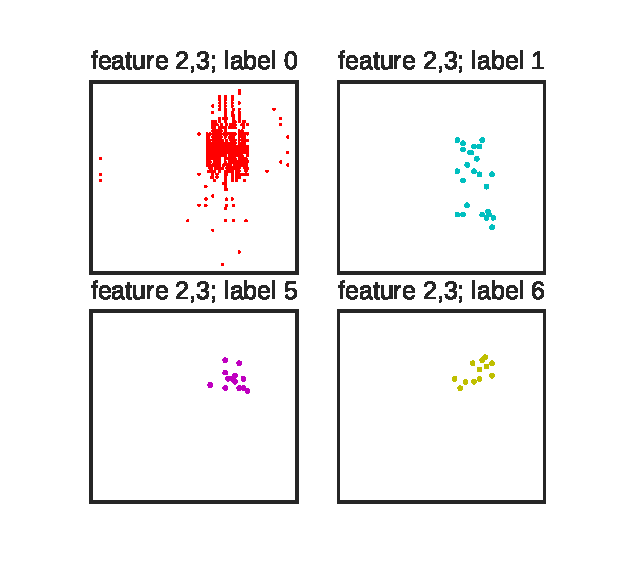
\includegraphics[scale=0.4, trim=0 0 0 0]{figs/data_features}\\
	\label{fig1}
	\figcaption{第0.1维特征分类图}
\end{center}

由图1可以看出8类故障中第一类故障也就是无故障类别所占比例很大,而第三、四、五类故障所占的比例相对第一类故障所占的比重要小很多,这是严重的不均衡分类问题,并且,故障分布较分散,不利于分类器进行分类。因此,问题处理过程中对于占比重较小的故障类对其分类正确率不作为评判指标。

\subsection{BP网络的建立}

首先,人工神经网络对于知识有较强的学习能力,它对数据的并行处理能力可大大提高其处理信息的能力的速度。基于这种思想,我们将神经网络技术应用于磨矿生产过程中的诊断,从而获得理想的诊断效果。

目前应用较多前馈型网络的是BP网络,其学习速度快,逼近能力和分类能力强,本文使用BP神经网络来对磨矿中的故障进行诊断,诊断系统功能结构见图2。

\begin{center}
	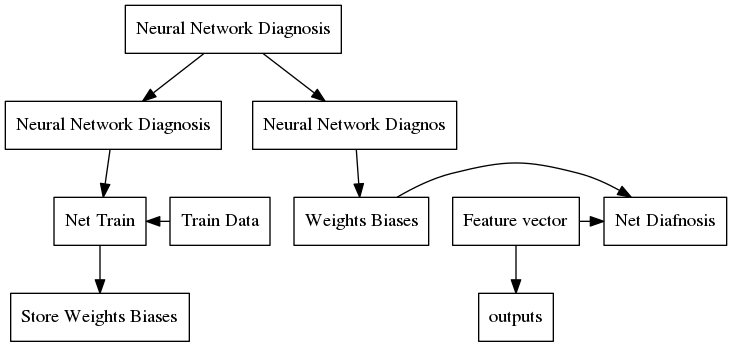
\includegraphics[scale=0.12, trim=0 0 0 0]{figs/procedure}
	\label{fig2}
	\figcaption{磨矿神经网络故障诊断功能示意图}
\end{center}

传统的BP神经网络,容易陷入局部极小点,本文采用“成批处理”的学习方法,这种方法在训练神经网络的过程中,不受学习样本排序的影响,使收敛速度加快;并采用了学习率自调整的方法。本文构建的BP神经网络的模型为,三层神经网络即输入层,隐层和输出层三层。在样本数据输入网络之前,由于数据之间不存在很大的相关性,且数量级之间存在较大的差异,所以本文将数据进行归一化处理后,再进行数据输入。

\subsection{实验与结果分析}

本文分别采用$1024\times24$维的整体数据集划分为$900\times24$维的数据作为训练样本集,剩下的$124\times24$维数据作为测试集,进行验证可以防止网络过拟合。在训练样本集输入到网络时,进行分批处理,即每次输入$32\times24$维的数据,训练好网络后保存其权重和阈值,测试集再输入到训练好的网络中,来验证网络可靠性和诊断的准确率。

训练样本集输入后网络的输出从大的层面上讲分为两类:一是有无故障,二是有故障;对于有故障的接下来进行进一步的分析是哪一类故障。本文中的故障辨识问题不是传统的分类问题,其存在着严重的分类不均衡问题。在非均衡分类中的主要评价指标可以利用混淆矩阵给出,如表2所示。


\begin{center}
	\tabcaption{混淆矩阵表}
	\label{tab:2}
	\begin{tabular} {cccc}\toprule
		\multirow{2}{*}[-2pt]{}&\multirow{2}{*}[-2pt]{}&\multicolumn{2}{c}{预测结果}\\
		\cmidrule(lr){3-4}
		&&$+1$&$-1$\\\hline
		\multirow{2}{*}[-2pt]{真实结果}&$+1$&真正例(TP)&伪反例(FN)\\
		&$-1$&伪正例(FP)&真反例(TN)\\
		\bottomrule
\end{tabular}\end{center}

这里以简单的二值分类问题进行说明,在二值分类问题中,如果将一个整理判为正例,那么就认为产生了一个真正例(True Positive,TP,也称真阳);如果对一个反例正确的判为反例,则认为产生了一个真反例(True Negative,TN,也称真阴)。相应地,另外两种情况则分别称为伪反例(Flase Negative,FN,也称假阴)和伪正例(False Positive,FP,也称假阳),这四种情况如表2所示。

在分类问题中,当某个类别的重要性高于其他类别时或者存在不均衡分类时,我们就可以利用上述定义来构造出多个比错误率更加适合作为衡量标准的新指标。

本文中将有故障当作正例,没有故障当作反例,定义了如下评价指标:

(1)错误率$S_1$:
\begin{align}
S_1=1-\frac{TP+TN}{TP+FP+TN+FN}
\end{align}

这个指标对于不存在非均衡分类和当某个类别的重要性高于其他类别时较为实用,在本问题中不是特别适合,仅为一个参考评价指标。

(2)预测有故障正确率$S_2$(正例正确率):
\begin{align}
S_2=\frac{TP}{TP+FP}
\end{align}

这个指标给出的是预测为正例样本中的真正例的比例。若在本次实验中分类器对数据集进行预测分类时得出$N$个样例为有故障类别;且在这$N$个预测有故障的类别里面有$n$个是真正的有故障类别,那么正例正确率即预测有故障正确率为$n/N$。

(3)预测无故障正确率$S_3$(反例正确率):
\begin{align}
S_3=\frac{TN}{TN+FN}
\end{align}

这个指标给出的是预测为反例的样本中真正反例的比例。若在本次实验中分类器对数据集进行预测分类时得出$M$个样例为有故障类别,且在这$M$个预测有故障的类别里面有$m$个是真正的有故障类别,那么正例正确率即预测无故障正确率为$m/M$。

对传统的BP神经网络进行实验验证,实验结果如下:


\begin{center}
	\tabcaption{BP神经网络实验结果}
	\label{tab:3}
	\begin{tabular} {cccc}\toprule
		\multirow{2}{*}[-2pt]{}&\multirow{2}{*}[-2pt]{}&\multicolumn{2}{c}{预测结果}\\
		\cmidrule(lr){3-4}
		&&有故障&无故障\\\hline
		\multirow{2}{*}[-2pt]{真实结果}&有故障&21&24\\
		&无故障&24&55\\
		\bottomrule
\end{tabular}\end{center}

通过实验结果可以计算出不作任何特征变换的BP神经网络,神经元网络激活函数使用Sigmoid函数,节点大小为$24\rightarrow100\rightarrow8$,,对于预测有故障的正确率为46.7\%,无故障的正确率为69.6\%,错误率为38.7\%。可以看出,如果对于输入的特征向理想不作任何特征变化就输入到神经网络中,网络在有无故障的辨识正确率方面表现都比较差,并且错误率较高。这也进一步说明传统BP神经网络不适用高维输入的非均衡分类问题。

\section{原始自动编码器}

本文中的训练样本集的输入维数为24维,但是这样对于神经网络来说输入的维数越高对于神经网络的训练效果并不是太好,那么可以运用类似于图像无损压缩的技术对训练样本输入进行进一步的特征提取,恰好Autoencoder自编码神经网络就是一种很好的选择。

自编码神经网络是一种无监督学习算法,它让其输出值等于输入值。如果神经网络隐藏层神经元个数远小于输入层和输出层,这样就迫使自编码神经网络去学习输入数据的压缩表示,假设神经网络输入的数据是完全随机的数据,那么要学习这些随机数据的压缩表示是十分困难的;但是如果某些特征之间是彼此相关的,那么,自编码算法就能发现这些有联系数据间的相关性,并能在输出层重构出输入数据。相反,如果神经网络的隐层神经元个数较多或与输入层想当时,还可以对隐藏层神经元上加上稀疏性限制,这样自编码神经网络仍能发掘出输入数据之间的相关性。

本文建立了两个网络,一个为Autoencoder自编码神经网络,可以看作一个三层神经网络,输入数目与输出数目相同,隐藏层神经元个数为10少于输入个数,各层神经元的激活函数选为Sigmoid函数。其目的和PCA相似就是把输入的特征进行进一步的提取。另外一个就是前端与Autoencoder网络前两层相同,输出层接一个Softmax分类器就形成了AutoencoderSoftmax分类器网络。该网络的隐藏层的输出值正好就是类似池化后的特征值,但其几乎包含了输入向量的所有信息,输出层为9个神经元,正好为输出的9种故障类别。与传统神经网络不同的是,输出层的变为了一个Softmax分类器,网络的具体结构如图
3所示。

\begin{center}
	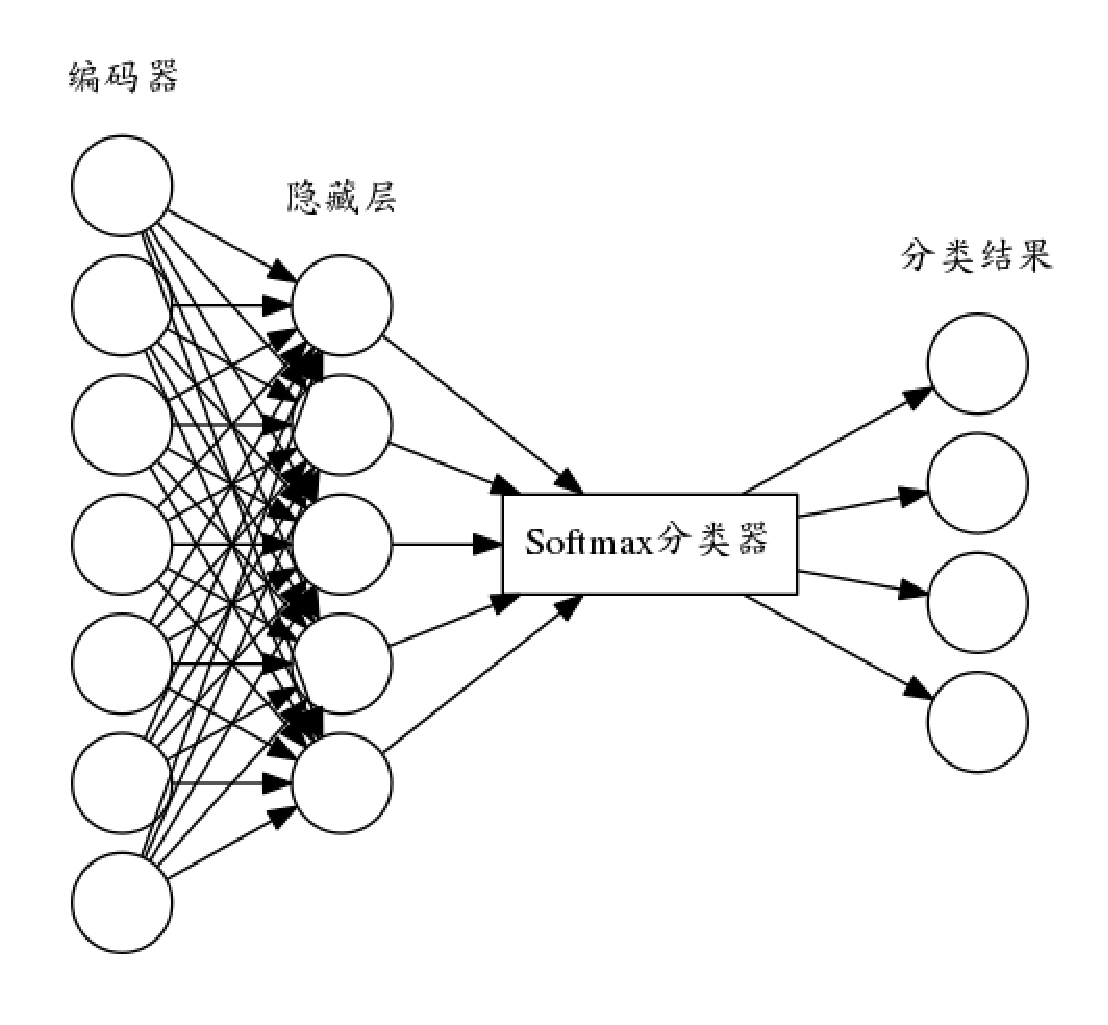
\includegraphics[scale=0.12, trim=0 0 0 0]{figs/autoencoder_softmax}\\
	\label{fig4}
	\figcaption{传统自动编码深度学习网络架构}
\end{center}

网络训练时分为两部分,首先对自动编码网络训练,将$24$维的训练样本集全部输入,按照BP网络的梯度下降算法进行训练使输出尽可能的与输入均方差最小。Autoencoder网络训练完,将最终的权重和阈值保存下来。接下来就是训练AutoencoderSoftmax分类器网络,将前面训练好的网络保存下来的权重和阈值来初始化新构建的神经网络的权值和阈值,重新进行训练。自编码网络结构为$24\rightarrow150\rightarrow24\rightarrow150\rightarrow24$,激活函数为RELU,此时训练的算法为L-BFGS,学习率为0.01,目标函数为使得“交叉熵”最小。交叉熵产生于信息论里面的信息压缩编码技术,是用来衡量我们的预测用于描述真相的低效性,使交叉熵越小也就是低效性越低即准确率越高。

\subsection{对比AutoencoderBP和AutoencoderSoftmax辨识效果}

在对BP网络和AutoencoderSoftmax深度学习网络进行实验时,选择其中909组数据作为训练样本集,余下的115组数据作为测试集来进行验证。

基于2.3提出几种分类评价标准,本文对AutoencoderBP神经网络和AutoencoderSoftmax深度学习网络进行对比测试实验。

在24维特征向量输入网络之前,利用Autoencoder自编码网络对其进行特征提取。自编码网络也可以看作一种神经网络,其目标函数就是使输出尽可能的与输入相等,这样既可以在隐含层实现无损压缩。为了验证自编码网络的性能我们选取其中八维特征观察还原效果如图4所示。

\begin{center}
	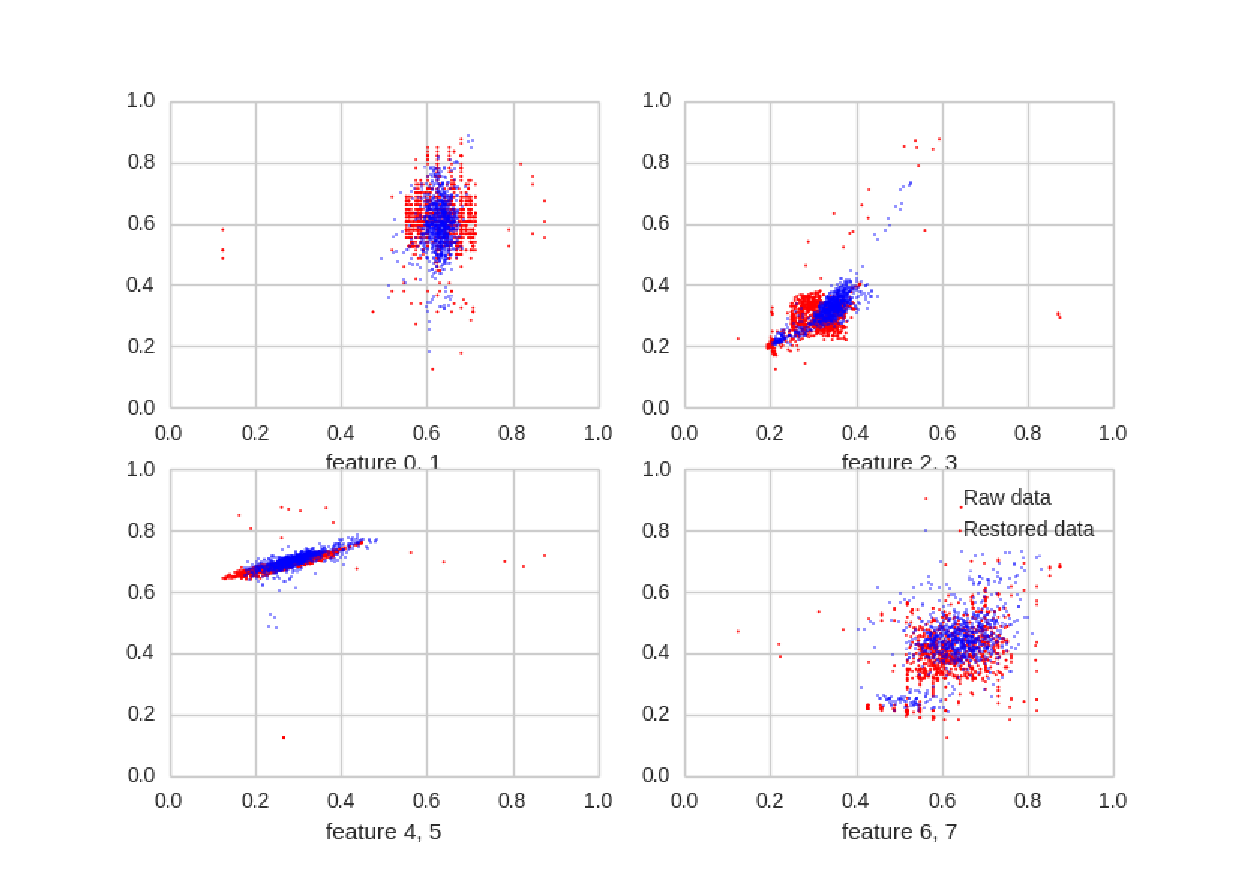
\includegraphics[scale=0.4, trim=0 0 0 0]{figs/autoencoder_restore}\\
	\label{fig5}
	\figcaption{自编码还原效果图}
\end{center}

由以上图可以看出,编码还原后绝大多数的特征点还是与编码前的特征点比较接近,因此可以看出,自编码网络经过多步训练后能够较好的复现输入也就是说隐含层提取到的特征包含了输入特征的大部分信息,即可以用隐含层的输出的更加明显的特征向量来代替原网络的高维输入向量。

训练完成后,获得编码后的隐藏层输出的特征如图5所示:

\begin{center}
	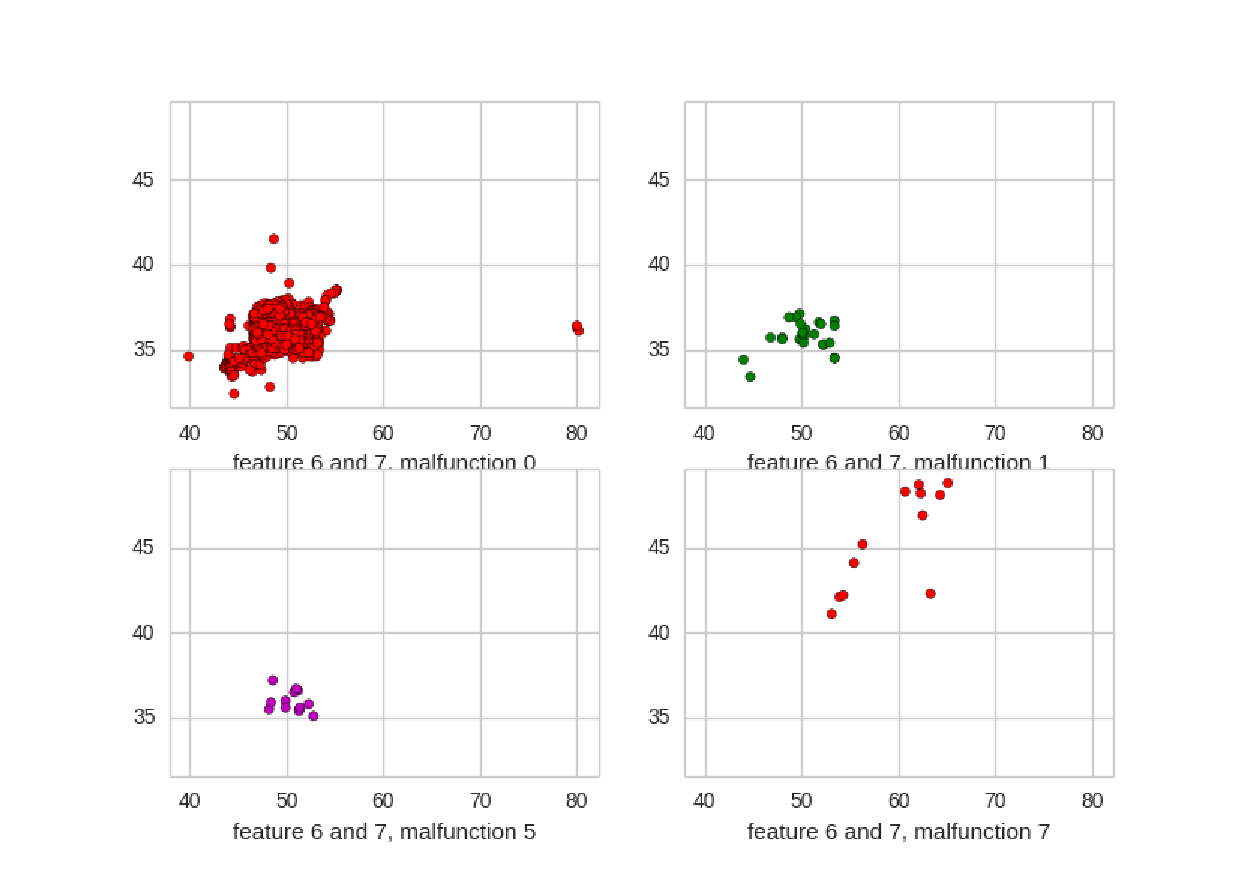
\includegraphics[scale=0.4, trim=0 0 0 0]{figs/autoencoder_encoded_features}\\
	\label{fig6}
	\figcaption{自编码网络输出特征}
\end{center}

由图5可以看出自编码后的特征较编码前的特征数量上大幅度下降,这正是自编码对高维冗余特征无损压缩使有效特征浮现的结果。不仅在特征数量上有所降低,而且故障点的分布较集中,这样就可以利用分类器实现准确的分类。

\paragraph{BP神经网络实验结果}

\begin{center}
	\tabcaption{AutoencoderBP实验结果}
	\label{tab:3}
	\begin{tabular} {cccc}\toprule
		\multirow{2}{*}[-2pt]{}&\multirow{2}{*}[-2pt]{}&\multicolumn{2}{c}{预测结果}\\
		\cmidrule(lr){3-4}
		&&有故障&无故障\\\hline
		\multirow{2}{*}[-2pt]{真实结果}&有故障&30&15\\
		&无故障&15&55\\
		\bottomrule
\end{tabular}\end{center}

由表4可以计算出AutoencoderBP网络对于有故障预测的准确率为66.7\%,而对于无故障预测的正确率为78.6\%,错误率也下降为26.1\%。可以看出,相较传统的BP神经网络其在有无故障预测的正确率方面有了一定提高,同时错误率也有所下降,特征经过自编码网络编码后,有效特征被提取出来,提高了传统BP网络的辨识能力。

\paragraph{AutoencoderSoftmax深度学习网络实验结果}

\begin{center}
	\tabcaption{AutoencoderSoftmax实验结果}
	\label{tab:3}
	\begin{tabular} {cccc}\toprule
		\multirow{2}{*}[-2pt]{}&\multirow{2}{*}[-2pt]{}&\multicolumn{2}{c}{预测结果}\\
		\cmidrule(lr){3-4}
		&&有故障&无故障\\\hline
		\multirow{2}{*}[-2pt]{真实结果}&有故障&37&8\\
		&无故障&8&62\\
		\bottomrule
\end{tabular}\end{center}

训练完自动编码器之后,在隐藏层特征之后加入Softmax分类器,得到最终分类网络结构为$24\rightarrow150\rightarrow24\rightarrow8$,利用表5中的数据带入上面的公式可以得到AutoencoderSoftmax深度学习网络预测有故障的正确率为82.2\%,预测无故障的正确率为88.5\%,而错误率降低为13.9\%。

由上述结果可知,AutoencoderSoftmax深度学习网络在预测有无故障正确率方面明显优于前面两种网络,此外还大大降低了错误率,由此可以看出该深度学习网络对分均衡分类问题有着良好的分类效果。

\section{引入DropOut与降噪自编码}
从图4也能看出,传统自动编码器对数据的恢复效果一般,而且使用测试集测试自动编码器编码的时候,编码效果明显弱于训练集。这是因为自动编码器对噪声数据有着一定的过拟合。为了解决这个困难,我们引入DropOut与降噪自编码技术。

\subsection{DropOut}
DropOut是一种通用的训练神经网络并能明显降低过拟合的方法。在训练过程中,将神经网络中的神经元按照一定概率$P(d)$丢弃,训练这些稀疏的模型,并去掉全职惩罚项,将其替换为限制权值的上限。因为噪声通常表现为高频干扰,用这种方法既可以将高频干扰钳位,又可以以较低成本实现模型融合的效果。在测试过程中,将输入校正为为$1-P(d)$倍,使得神经网络传输的数据均值不变。DropOut结构如图7所示。

\begin{center}
	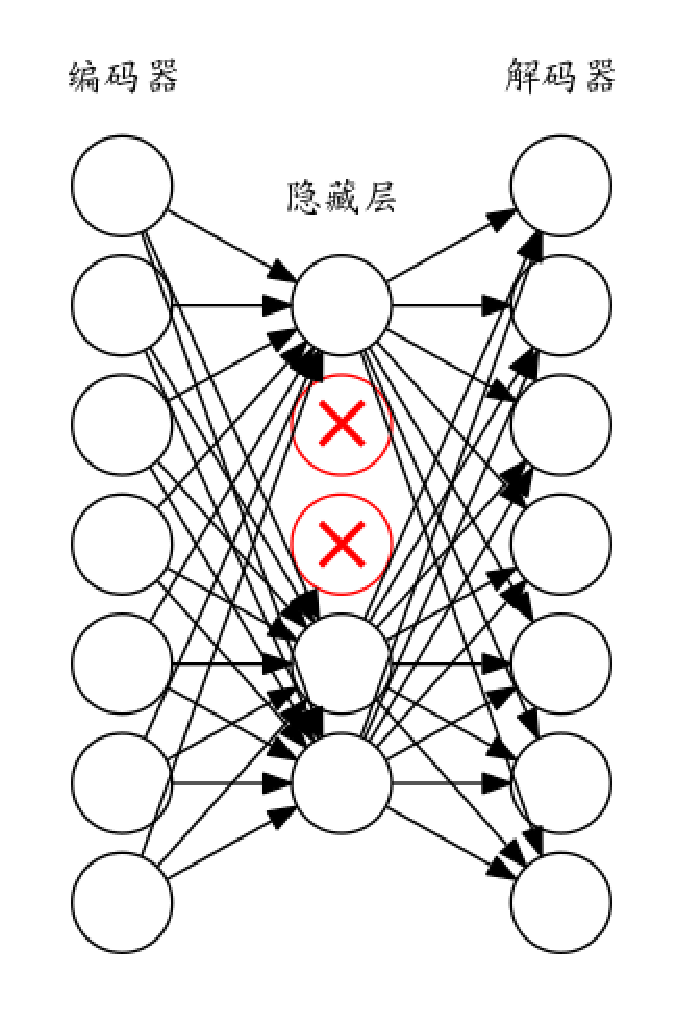
\includegraphics[scale=0.16, trim=0 0 0 0]{figs/dropout}\\
	\label{fig7}
	\figcaption{DropOut结构示意图}
\end{center}

\subsection{降噪自编码}
降噪自编码通过将输入数据加入随机干扰,或将输入数据的某些维度随机置零。训练时要求即便加入了干扰,仍够可以还原输入。通过这种方法,可以使自动编码器无监督地能学习到更加鲁棒的高层特征,克服噪声的干扰,显著减少神经网络对噪声的拟合。降噪自编码的结构示意图如图8所示。


\begin{center}
	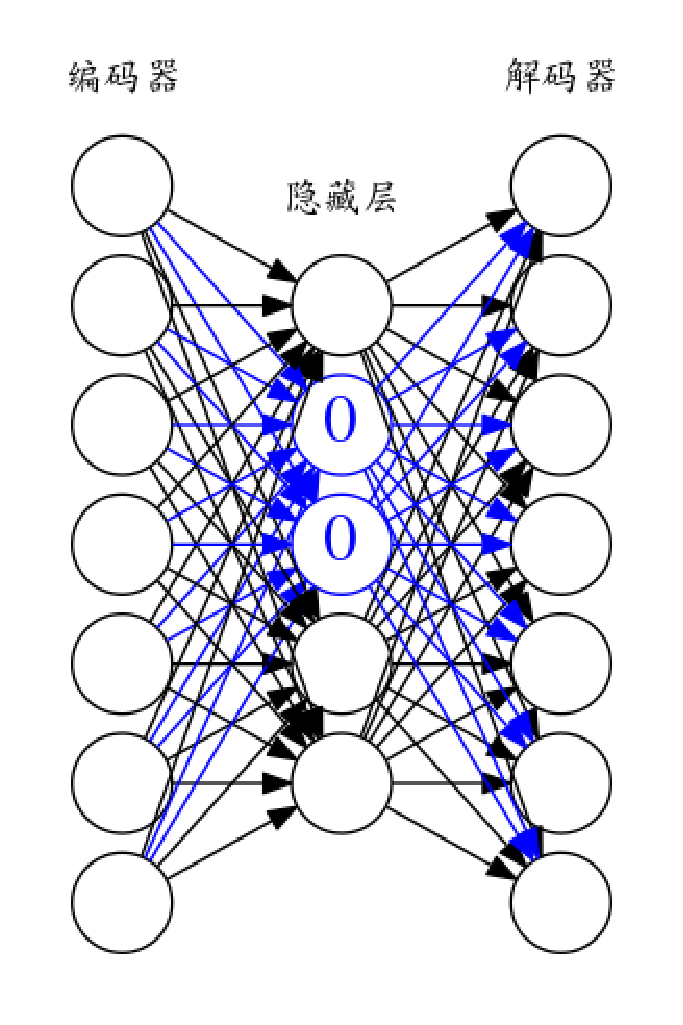
\includegraphics[scale=0.16, trim=0 0 0 0]{figs/denoised_autoencoder}\\
	\label{fig8}
	\figcaption{降噪自编码结构示意图}
\end{center}

\subsection{实验与结果分析}

在对自动编码器行实验时,选择909组数据作为训练样本集,余下的115组数据作为测试集来进行验证。为方便比较,使用与之前的自动编码器相同网络结构,将$24$维的训练样本集全部输入。自编码网络结构为$24\rightarrow150\rightarrow24\rightarrow150\rightarrow24$,训练完自动编码器之后,在隐藏层特征之后加入Softmax分类器,得到最终分类网络结构为$24\rightarrow150\rightarrow24\rightarrow8$。激活函数为RELU,训练的算法为L-BFGS,学习率为0.01,目标函数为使得“交叉熵”最小。

\paragraph{加入DropOut的自动编码器实验结果}

\begin{center}
	\tabcaption{加入DropOut的自动编码器实验结果}
	\label{tab:5}
	\begin{tabular} {cccc}\toprule
		\multirow{2}{*}[-2pt]{}&\multirow{2}{*}[-2pt]{}&\multicolumn{2}{c}{预测结果}\\
		\cmidrule(lr){3-4}
		&&有故障&无故障\\\hline
		\multirow{2}{*}[-2pt]{真实结果}&有故障&39&6\\
		&无故障&7&63\\
		\bottomrule
\end{tabular}\end{center}

由表5可以计算出加入DropOut 之后网络对于有故障预测的准确率为88.7\%,而对于无故障预测的正确率为84.8\%,错误率也下降为26.1\%。可以看出,相较传统的BP神经网络其在有无故障预测的正确率方面有了一定提高,同时错误率也有所下降,特征经过自编码网络编码后,有效特征被提取出来,提高了传统BP网络的辨识能力。

\paragraph{加入DropOut的降噪自编码实验结果}

\begin{center}
	\tabcaption{加入DropOut的降噪自编码实验结果}
	\label{tab:6}
	\begin{tabular} {cccc}\toprule
		\multirow{2}{*}[-2pt]{}&\multirow{2}{*}[-2pt]{}&\multicolumn{2}{c}{预测结果}\\
		\cmidrule(lr){3-4}
		&&有故障&无故障\\\hline
		\multirow{2}{*}[-2pt]{真实结果}&有故障&39&6\\
		&无故障&5&65\\
		\bottomrule
\end{tabular}\end{center}

利用表5中的数据带入上面的公式可以得到AutoencoderSoftmax深度学习网络预测有故障的正确率为90.4\%,预测无故障的正确率为88.5\%,而错误率降低为13.9\%。

由上述结果可知,AutoencoderSoftmax深度学习网络在预测有无故障正确率方面明显优于前面两种网络,此外还大大降低了错误率,由此可以看出该深度学习网络对分均衡分类问题有着良好的分类效果。

\section{Conclusion}

本文提出的AutoencoderSoftmax深度学习网络能够很好的在繁冗的特征向量数据集中提取出有效特征并将输入数据的维数进行压缩,这样大大降低了网络的运算量。在非均衡分类问题中,传统的BP神经网络对于故障的辨识效果并不好,而且收敛速度较慢、容易陷入局部极小值,虽然采用了``成批处理''的方法收敛速度加快,但是辨识效果没有明显提高。相反,AutoencoderSoftmax深度学习网络尤其针对非传统分类问题,其收敛速度和辨识效果都要好于传统的BP网络。然而,由于传统的自动编码器对噪声数据有着过多拟合,提取到了许多不重要的特征,分类准确率还是难以令人满意。本文接下来使用加入DropOut 的降噪自编码,显著降低了分类错误率,达到工业界最先进的水平。这种方法将为今后的非传统分类问题提供一个理论依据,并将在深度学习实现故障辨识领域产生深远意义。


\bibliographystyle{bib/gbt7714-2005}
\bibliography{bib/reference.bib}
\editor{X~~~~X}
\end{multicols}
\end{document}


% \begin{thebibliography}{99}
%   %段落之间的竖直距离
% %1
% %{\renewcommand{\baselinestretch}{1.02}\selectfont
% \addtolength{\itemsep}{-0.7em}
% \bibitem[1]{1}刘于之,李木国,杜海.\;具有时延和丢包的NCS鲁棒 $H_{\infty}$控制[J].\;控制与决策, 2014, 29(3): 517-522.\\
% (Liu Y Z, Li M G, Du H. Robust $H_{\infty}$ control of NCS with delay and packet dropout[J]. Control and Decision, 2014, 29(3): 517-522.)
% %2
% \bibitem[2]{2}Zhu X L, Yue D. Stability of sampled-data systems with application to networked control systems[C]. Proc of the 32nd Chinese Control Conf. Xi'an: IEEE, 2013: 6572-6577.
% %3
% \bibitem[3]{3}Zhang C K, Jiang L, He Y, et al. Stability analysis for control systems with aperiodically sampled data using an augmented Lyapunov functional method[J]. IET Control Theory and Applications, 2013, 7(9): 1219-1226.
% %4
% \bibitem[4]{4}Seuret A, Briat C, Gouaisbaut F. Stability analysis of asynchronous sampled-data systems with discrete-time constant input delay[C]. Proc of the 53rd IEEE Conf on Decision and Control. Los Angeles: IEEE, 2014: 4342-4347.
% %5
% \bibitem[5]{5}Fujioka H. A discrete-time approach to stability analysis of systems with aperiodic sample-and-hold devices[J]. IEEE Trans on Automatic Control, 2009, 54(10): 2440-2445.
% %6
% \bibitem[6]{6}Naghshtabrizi P, Hespanha J P, Teel A R. Exponential stability of impulsive systems with application to uncertain sampled-data systems[J].  Systems \&  Control Letters, 2008, 57(5): 378-385.
% %7
% \bibitem[7]{7}Fridman E. A refined input delay approach to sampled-data control[J].  Automatica, 2010, 46(2): 421-427.
% %8
% \bibitem[8]{8}Liu K, Fridman E. Wirtinger's inequality and Lyapunov-based sampled-data stabilization[J].  Automatica, 2012, 48(1): 102-108.
% %9
% \bibitem[9]{9}Shao H Y, Han Q L, Zhang Z Q, et al. Sampling-interval-dependent stability for sampled-data systems with state quantization[J].  Int J of Robust Nonlinear Control, 2014, 24(17): 2995-3008.
% %10
% \bibitem[10]{10}Shao H Y, Lam J, Feng Z G. Sampling-interval-dependent stability for linear sampled-data systems with non-uniform sampling[J]. Int J of Systems Science, 2016, 47(12): 2893-2900.
% %11
% \bibitem[11]{11}Seuret A. A novel stability analysis of linear systems under asynchronous samplings[J]. Automatica, 2012, 48(1): 177-182.
% %12
% \bibitem[12]{12}Seuret A, Gouaisbaut F. Wirtinger-based integral\linebreak     inequality: Application to time-delay systems[J]. Automatica, 2013, 49(9): 2860-2866.
% %13
% \bibitem[13]{13}Gu K. An integral inequality in the stability problem of time-delay systems[C]. Proc of the 39th IEEE Conf on Decision and Control. Sydney: IEEE, 2000: 2805-2810.

% \end{thebibliography}\vspace{-20pt}


